\section{Introduction}

\textit{Cyber-physical systems} (CPSs)  are integration of computation with physical processes whose behavior is defined by both computational and physical parts of the system \cite{Zanero17}. Embedded computers and networks monitor and control the physical processes, usually with feedback loops where physical processes affect computations and vice versa. The heterogeneity is one of the main characteristics of CPSs. The components of CPSs are of various types, requiring interfacing and interoperability across multiple platforms and different models of computation. Verification of CPSs as a whole requires the use of heterogeneous simulation environments. One emerging industry
standard is the Functional Mock-up Interface (FMI) \cite{Blochwitz2011The}. It
is a standard designed to support simulation of complex systems
comprising heterogeneous components, by coupling the different models with their own solver in a co-simulation environment.

FMI \cite{BromanBGLMTW13} defines an standard applied to composing model components which are designed with different modeling tools. The FMI standard was first developed in the MODELISAR project started in 2008 and supported by a large number of software companies and research centers. FMI offers the means for model based development of systems and is particularly appropriate way to develop complex CPSs. The FMI standard supports both co-simulation and  model exchange. However, in this paper, we focus on the co-simulation in FMI 2.0.
Compared with the FMI 1.0, there are two important additions: \emph{fmiGetFMUstate} and \emph{fmiSetFMUstate}, which allow the master to copy and later restore the complete state of an FMU slave. These two functions provide an ordinary mechanism for rollback. The function \emph{fmiDoStep} is to determine the execution step size of FMU, called by the MA to orchestrate the exchange of data among the FMUs during the entire co-simulation. 

\emph{fmiStatus fmiDoStep (fmiComponent c, fmiReal currentCommunicationPoint, fmiReal communicationStepSize, fmiBoolean noSetFMUStatePriorToCurrentPoint);}

The \emph{currentCommunicationPoint} argument is the current communication time of the master. The \emph{communicationStepSize} is the time step that the master proposes to the slave. Given a time step, the slave may accept or reject the step. For example, it may reject it because the step size is so large that causes a discrete event within the step. If the argument \emph{noSetFMUStatePriorToCurrentPoint} is true, the master will no longer call \emph{fmiSetFMUstate} for time instants prior to \emph{currentCommunic tionPoint} in this simulation run. 

Master algorithm(MA) \cite{AckerDVM15} provides the orchestration of the entire co-simulation. However, the master algorithm is not part of the FMI standard. This implies that the user or tool vendor needs to develop a sophisticated orchestration algorithm for the problem at hand. The correctness of the master algorithm also needs to be analysed. In this paper, we verify three versions of master algorithms \cite{BromanBGLMTW13}: fix step algorithm, rollback algorithm, predictable step size algorithm. Rollback and predictable step size algorithms are based on the extension of FMI 2.0, which supports the rollback and predict function. PG Larsen et al. \cite{Larsen2016Integrated} 
formally analysed the fix step and rollback algorithms with the FDR3 refinement checker. We model three versions of master algorithms with timed automata, and verify the algorithms with UPPAAL. Once the correctness of master algorithm is ensured, in the remainder of paper we model the co-simulation of CPSs to model check several properties of co-simulation such as deadlock, liveness, and reachability. 
To achieve the goal, we present a novel approach to model and verify the properties of co-simulation with timed automata \cite{AlurD94}. The schematic view of our approach is shown in Fig.\ref{paperarc}.
At the design phase, we construct the architecture of CPSs with SysML block diagrams \cite{RahimHI17}. Each block represents a component and the communication between components is modeled with SysML connector. To simulate the whole system with co-simulation techniques, the block can be modeled with a Functional Mock-up (FMU) and the connector can be modeled with a master algorithm. The MA orchestrate FMUs to accomplish the communication between FMUs. To verify the correctness of the architecture, we encode the FMU and the master algorithm by timed automata, which facilitates the verification livelock or deadlock with the model checker UPPAAL \cite{BehrmannDLHPYH06}.
\begin{figure}[htbp]
	\centering	{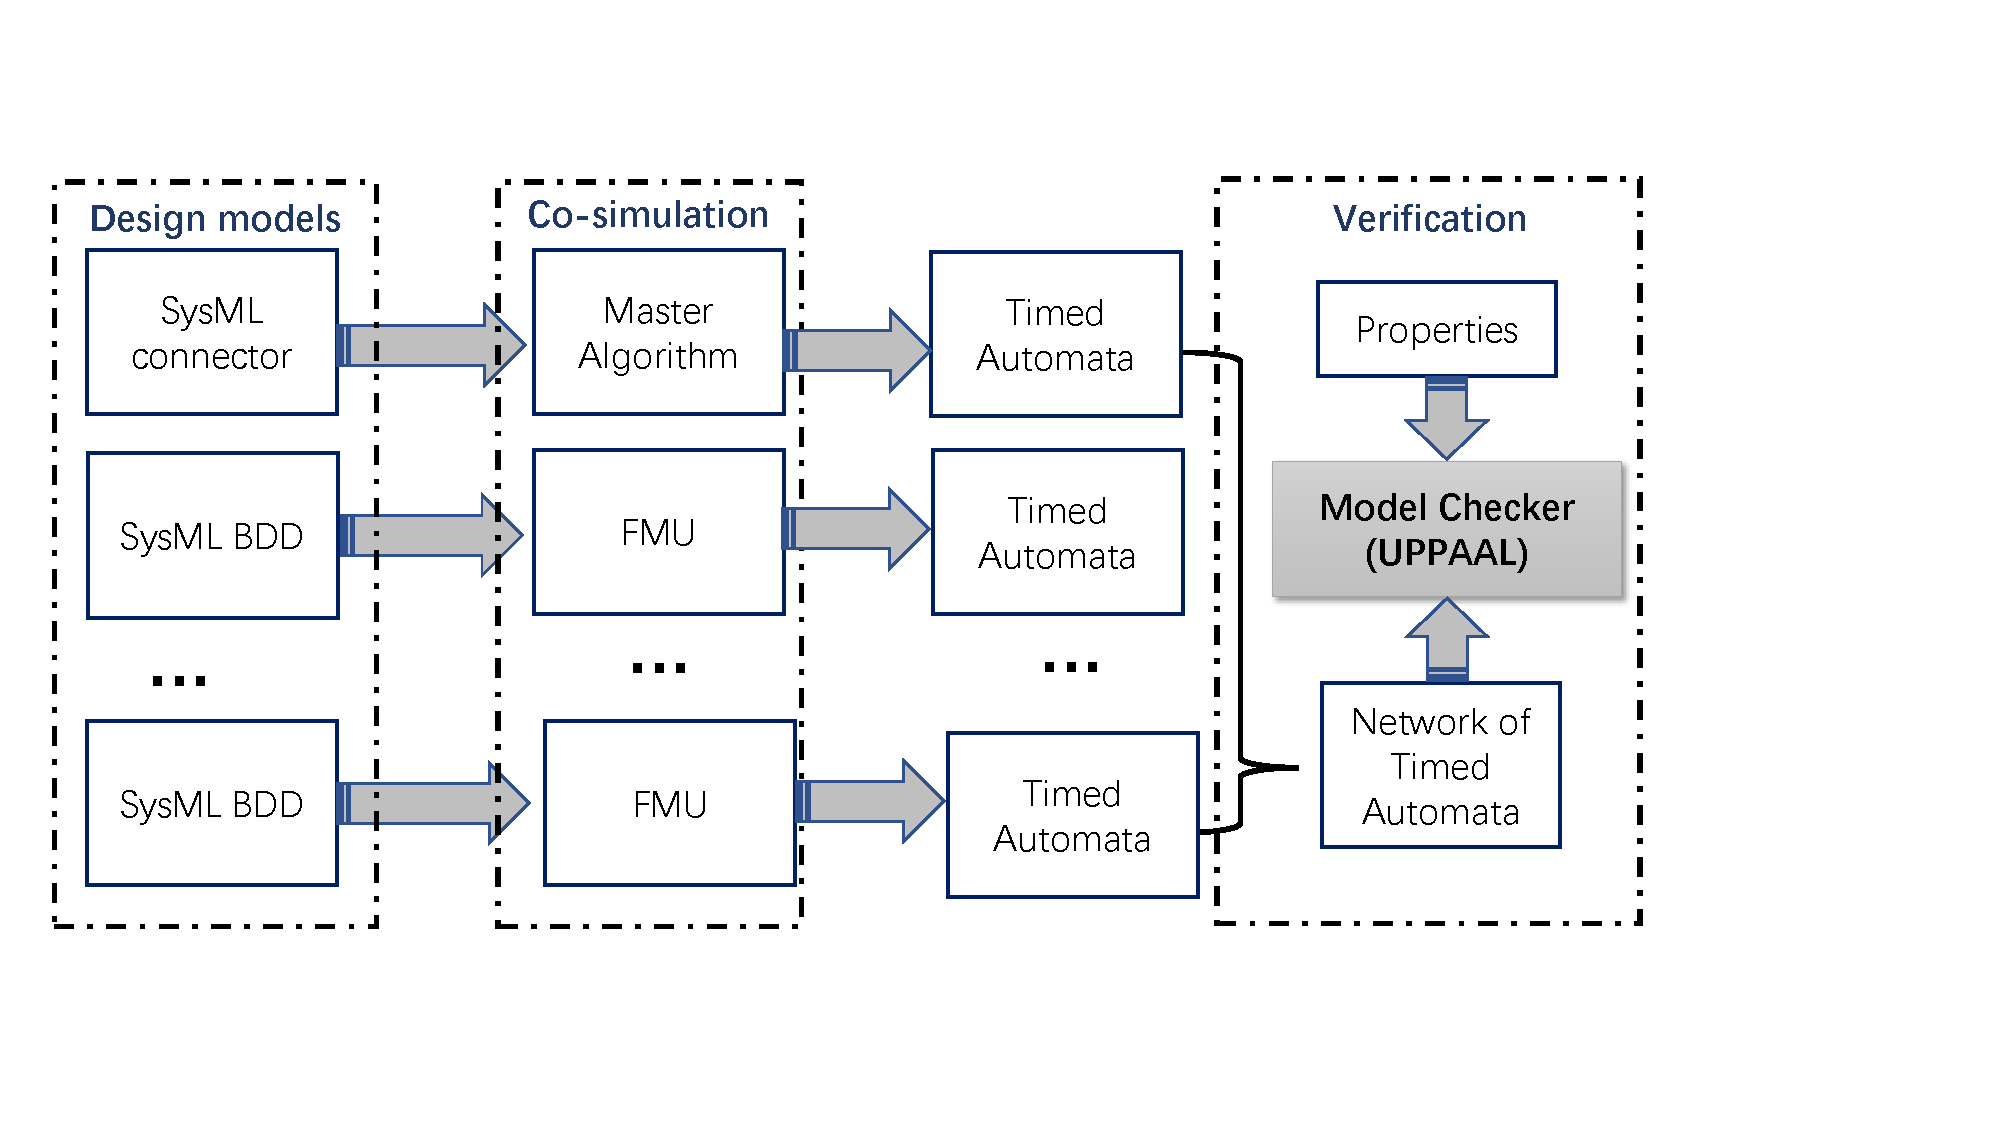
\includegraphics[width=3.5in,height=1.6in]{fig/approach.pdf}}
	\caption{A schematic view of our approach.}
	\label{paperarc}
\end{figure}

\textbf{Contributions.} Our contributions are as follows:
\begin{itemize}
\item
We present a novel approach to model checking several properties of the co-simulation, such as livelock, deadlock and reachability. Moreover, we propose to check the absence of algebraic loops of SysML architectural model.
\item
We model the master algorithms for co-simulation with timed automata. Three various master algorithms are analysed with model checking. Besides, FMU is also modeled with timed automata and the orchestration between FMUs is modeled with a network of timed automata. With the help of UPPAAL, we analyse the reachability, livelock and deadlock of the architecture.
\item
We present how to model the architecture of CPSs with SysML block diagrams. We deal with the heterogeneity of CPSs by supporting multi-modelling and co-simulation based on FMI standard.
\item
The prototype for model checking co-simulation of CPSs is developing, which is integrated in our Mondana platform \cite{Cheng2015Modana}(https://github.com/ECNU-MODANA/AL-Modana.git). We have developed the SysML modelling environment and the \textit{co-simulator }for simulating CPSs\cite{Fritzson1998Modelica}.
\end{itemize}
The remainder of this paper is organized as follows. In Section~\ref{sec:fmi}, we briefly review the technical background including FMI, FMU and timed automata, and then provide encoding FMU by timed automata.
Section~\ref{sec:ma} models three versions of master algorithms with timed automata and verify the livelock and deadlock of three master algorithms.
Section~\ref{sec:sysml} presents the architecture modelling with SysML block diagrams.
Section~\ref{sec:ma&uppaal} presents the model checking FMI co-simulation with the example water tank. The experimental results show that our approach is feasible and useful. 
Finally we position our work with respect to related work before concluding and discussing possible future extensions.




















%The syntax of TA is as follows:
%\par
%\textbf{Timed Automata}
%A timed automata over a finite set of clocks $C$ and a finite set of actions $Sigma$ is a quintuple $\textit{H}=(L,l_{0},\Sigma,E,I)$, where
%\begin{itemize}
%\item
%$L$ is a finite set of locations,
%\item
%$l_{0}\in L$ is the initial location,
%\item
%$\Sigma$ is a finite set of actions, and $\Sigma=\Sigma_{i}+\Sigma_{o}$, where $\Sigma_{i}$ is the set of input actions, $\Sigma_{o}$ is the set of output actions,
%\item
%$E$ is a finite set of transactions, where $E\subseteq L \times \mathcal{B(C)}\times \Sigma \times 2^C\times L$
%\item
%$I:L\rightarrow \mathcal{B(C)})$ assigns invariants to locations.
%\end{itemize}